\documentclass{standalone}
\usepackage{tikz}

\begin{document}
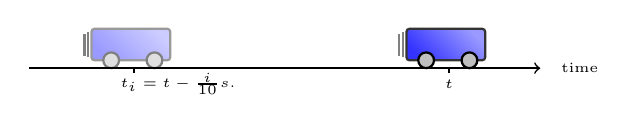
\begin{tikzpicture}
  \begin{scope}[scale=0.2]
    \shade[
        top color=blue!40, bottom color=blue!20, shading angle={135}
        ][
        draw=black!40,rounded corners=0.25ex,thick
        ] (1.5,.5) rectangle (6.5,2.5);
    % Wheels
    \draw[draw=black!50,fill=gray!25,thick] (2.75,.5) circle (.5);
    \draw[draw=black!50,fill=gray!25,thick] (5.5,.5) circle (.5);
    % Speed
    \draw[draw=black!50, thick] (1.275,.7) -- (1.275,2.3);
    \draw[draw=black!50, thick] (1.05,.8) -- (1.05,2.2);
    % Tick
    \draw[semithick] (4.20,0) -- (4.20,-0.3);
    \draw (7,-1) node {\tiny $t_i = t - \frac{i}{10}s.$};
  \end{scope}

  \begin{scope}[scale=0.2]
  \shade[
        top color=blue!80, bottom color=blue!40, shading angle={135}
        ][
        draw=black!80,rounded corners=0.25ex,thick
        ] (21.5,.5) rectangle (26.5,2.5);
    % Wheels
    \draw[draw=black,fill=gray!50,thick] (22.75,.5) circle (.5);
    \draw[draw=black,fill=gray!50,thick] (25.5,.5) circle (.5);
    % Speed
    \draw[draw=black!50, thick] (21.275,.7) -- (21.275,2.3);
    \draw[draw=black!50, thick] (21.05,.8) -- (21.05,2.2);
    % Tick
    \draw[semithick] (24.20,0) -- (24.20,-0.3);
    \draw (24.2,-1) node {\tiny $t$};
  \end{scope}
  
  \draw[->,semithick] (-.5,0) -- (6,0);
  \draw (6.5,0) node {\tiny time};
\end{tikzpicture}
\end{document}
